\documentclass[preview]{standalone}

\usepackage{amsmath}
\usepackage{amssymb}
\usepackage{bettelini}
\usepackage{stellar}
\usepackage{wrapfig}
\usepackage{definitions}

\begin{document}

\id{measuretheory-completed-product-measures}
\genpage

\section{Measurability Is Essential}

\begin{snippetexample}{iterable-sections-do-not-imply-product-measurability}{An iterated integral may exist for a nonmeasurable function}
    \begin{wrapfigure}{r}{6cm}
        \begin{center}
            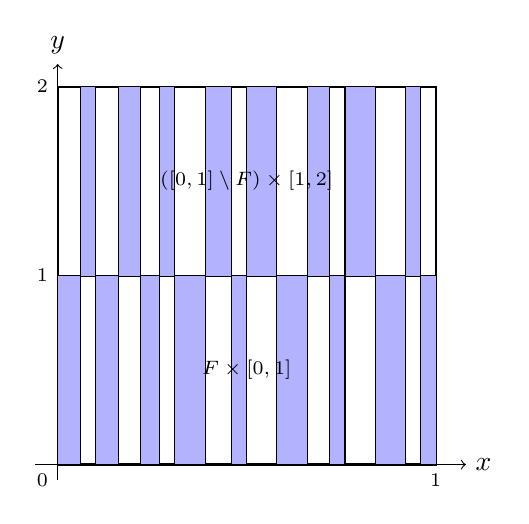
\begin{tikzpicture}[x=4.8cm,y=2.4cm]
                \draw[thick] (0,0) rectangle (1,2);
                \draw[thick] (0,1) -- (1,1);
                \foreach \a/\b in {0.00/0.06,0.10/0.16,0.22/0.27,0.31/0.39,0.46/0.50,0.58/0.66,0.72/0.76,0.84/0.92,0.96/1.00}{
                    \fill[blue!30] (\a,0) rectangle (\b,1);
                }
                \foreach \a/\b in {0.06/0.10,0.16/0.22,0.27/0.31,0.39/0.46,0.50/0.58,0.66/0.72,0.76/0.84,0.92/0.96}{
                    \fill[blue!30] (\a,1) rectangle (\b,2);
                }
                \foreach \x in {0.06,0.10,0.16,0.22,0.27,0.31,0.39,0.46,0.50,0.58,0.66,0.72,0.76,0.84,0.92,0.96}{
                    \draw[thin] (\x,0) -- (\x,2);
                }
                \draw[->] (-0.06,0) -- (1.08,0) node[right] {$x$};
                \draw[->] (0,-0.08) -- (0,2.12) node[above] {$y$};
                \node[below left] at (0,0) {\scriptsize $0$};
                \node[below] at (1,0) {\scriptsize $1$};
                \node[left] at (0,1) {\scriptsize $1$};
                \node[left] at (0,2) {\scriptsize $2$};
                \node at (0.5,0.5) {\scriptsize $F\times[0,1]$};
                \node at (0.5,1.5) {\scriptsize $\left([0,1]\setminus F\right)\times[1,2]$};
            \end{tikzpicture}
        \end{center}
    \end{wrapfigure}
    Let \(F\subseteq[0,1]\) be non-Lebesgue-measurable and define
    \[
        E=
        \bigl(F\cartesianprod[0,1]\bigr)
        \cup
        \bigl(([0,1]\setminus F)\cartesianprod[1,2]\bigr).
    \]
    For \(0<y<1\), \(E^y=F\), and for \(1<y<2\),
    \(E^y=[0,1]\setminus F\). Therefore \(E\) does not belong to the product
    \(\sigma\)-algebra and \(\chi_E\) is not product measurable.

    Nevertheless, every vertical section \(E_x\) is an interval of length
    one. Thus integration in the vertical direction can be completed:
    \[
        \int_0^1\left(\int_0^2\chi_{E_x}(y)\,dy\right)dx
        =\int_0^1 1\,dx=1.
    \]
    In the reverse order, the inner integrals are not defined because the
    horizontal sections are nonmeasurable. Hence the existence of one
    iterated integral says nothing by itself about product measurability.
    \wrapfill
\end{snippetexample}

\section{The Product of Complete Measures}

\begin{snippetproposition}{product-of-complete-measures-may-not-be-complete}{A product of complete measures need not be complete}
    Even if \(\mu\) and \(\lambda\) are complete, their product measure
    \(\mu\times\lambda\) need not be complete.
\end{snippetproposition}

\begin{snippetproof}{product-of-complete-measures-may-not-be-complete-proof}{product-of-complete-measures-may-not-be-complete}{A product of complete measures need not be complete}
    Suppose that \(\mu(\{x_0\})=0\) and that \(F\subseteq Y\) is not
    \(\lambda\)-measurable. The set
    \(\{x_0\}\cartesianprod F\) is not product measurable, since its section
    at \(x_0\) is \(F\). On the other hand,
    \[
        \{x_0\}\cartesianprod F
        \subseteq
        \{x_0\}\cartesianprod Y
    \]
    and
    \[
        (\mu\times\lambda)(\{x_0\}\cartesianprod Y)
        =\mu(\{x_0\})\lambda(Y)=0,
    \]
    with the usual convention \(0\cdot+\infty=0\). Thus a product-null set
    has a nonmeasurable subset.
\end{snippetproof}

\begin{snippettheorem}{euclidean-lebesgue-measure-product-completion}{Lebesgue measure is the completion of the product measure}
    Let \(n=a+b\). Lebesgue measure on \(\realnumbers^n\) is the completion
    of the product of Lebesgue measure on \(\realnumbers^a\) and Lebesgue
    measure on \(\realnumbers^b\).
\end{snippettheorem}

\begin{snippet}{completed-product-sigma-algebra-notation}
    We denote the completion of
    \(\mathcal M\cartesianprod\mathcal S\) with respect to
    \(\mu\times\lambda\) by
    \[
        (\mathcal M\cartesianprod\mathcal S)^*,
    \]
    and the completed measure by \((\mu\times\lambda)^*\).
\end{snippet}

\section{Fubini--Tonelli on the Completion}

\begin{snippettheorem}{fubini-tonelli-completed-product-measure-theorem}{Fubini--Tonelli for a completed product measure}
    Let \((X,\mathcal M,\mu)\) and \((Y,\mathcal S,\lambda)\) be complete,
    \(\sigma\)-finite measure spaces.
    \begin{enumerate}
        \item Let
            \(f\colon X\cartesianprod Y\fromto[0,+\infty]\) be measurable
            with respect to
            \((\mathcal M\cartesianprod\mathcal S)^*\). Then \(f_x\) is
            \(\mathcal S\)-measurable for almost every \(x\), and \(f^y\) is
            \(\mathcal M\)-measurable for almost every \(y\). After defining
            the exceptional sections arbitrarily, the corresponding
            integral functions are measurable and
            \[
                \int_{X\cartesianprod Y}f\,d(\mu\times\lambda)^*
                =
                \int_X\left(\int_Yf_x\,d\lambda\right)d\mu
                =
                \int_Y\left(\int_Xf^y\,d\mu\right)d\lambda.
            \]
        \item If
            \(f\in\mathcal L^1((\mu\times\lambda)^*)\), then its sections are
            integrable almost everywhere, the two integral functions are
            integrable, and the same equality holds.
    \end{enumerate}
\end{snippettheorem}

\begin{snippet}{completed-product-sections-almost-everywhere}
    Applying the completed theorem to \(f=\chi_E\) shows that if
    \(E\in(\mathcal M\cartesianprod\mathcal S)^*\), then almost every section
    of \(E\) is measurable in the corresponding factor. Unlike the
    uncompleted product case, measurability of every individual section is
    not guaranteed.
\end{snippet}

\end{document}
